\chapter{Technische Grundlagen und verwendete Werkzeuge}
\label{kap:grundlagen}
% Autor: Sebastian Lehner | Umfang-Ziel: ca. 9 Seiten

Dieses Kapitel erklärt die Technologien und Werkzeuge, die im Projekt verwendet wurden. Es beschreibt jeweils, \emph{was} ein Werkzeug ist und \emph{wofür} es gebraucht wurde. \emph{Wie} es konkret eingesetzt wurde, steht in den Kapiteln~\ref{kap:architektur-iteration} und~\ref{kap:implementierung}.

% ------------------------------------------------------------------
\section{Entwicklungsumgebung}
\label{sec:ide}

Eine Entwicklungsumgebung (IDE, \emph{Integrated Development Environment}) vereint Editor, Debugger, Terminal und Versionsverwaltung in einem Programm~\cite{pi-ide}.

Für das Backend wurde \textbf{WebStorm} von JetBrains verwendet, sowohl für das Admin-Package (\texttt{stack24-middleware-admin}) als auch in Projekt~A. WebStorm ist eine kostenpflichtige IDE für JavaScript und TypeScript mit Code-Vervollständigung, Refactoring-Werkzeugen und eingebautem Debugger~\cite{webstorm}. Gewählt wurde sie, weil sie bei Reichl und Partner Digital die am häufigsten verwendete IDE ist und Kollegen so direkt in derselben Umgebung helfen konnten. Für das Frontend wurde \textbf{Visual Studio Code} verwendet, ein kostenloser Editor von Microsoft, der über Erweiterungen ausgebaut werden kann~\cite{vscode}.

Beide zeigen Typfehler schon beim Tippen an, erlauben Debugging mit Breakpoints und haben eine eingebaute Git-Anbindung (Abbildung~\ref{fig:webstorm}). Für einheitlichen Code sorgen außerdem \textbf{ESLint}, das typische Fehler wie unbenutzte Variablen findet~\cite{eslint}, und \textbf{Prettier}, das den Code automatisch formatiert~\cite{prettier}. Beide werden über \texttt{pnpm lint} bzw. \texttt{pnpm format} aufgerufen.

\begin{figure}[htbp]
  \centering
  \begin{tikzpicture}
    % rechter Teil (leeres KI-Chat-Fenster) abgeschnitten
    \node[anchor=south west, inner sep=0] (img) {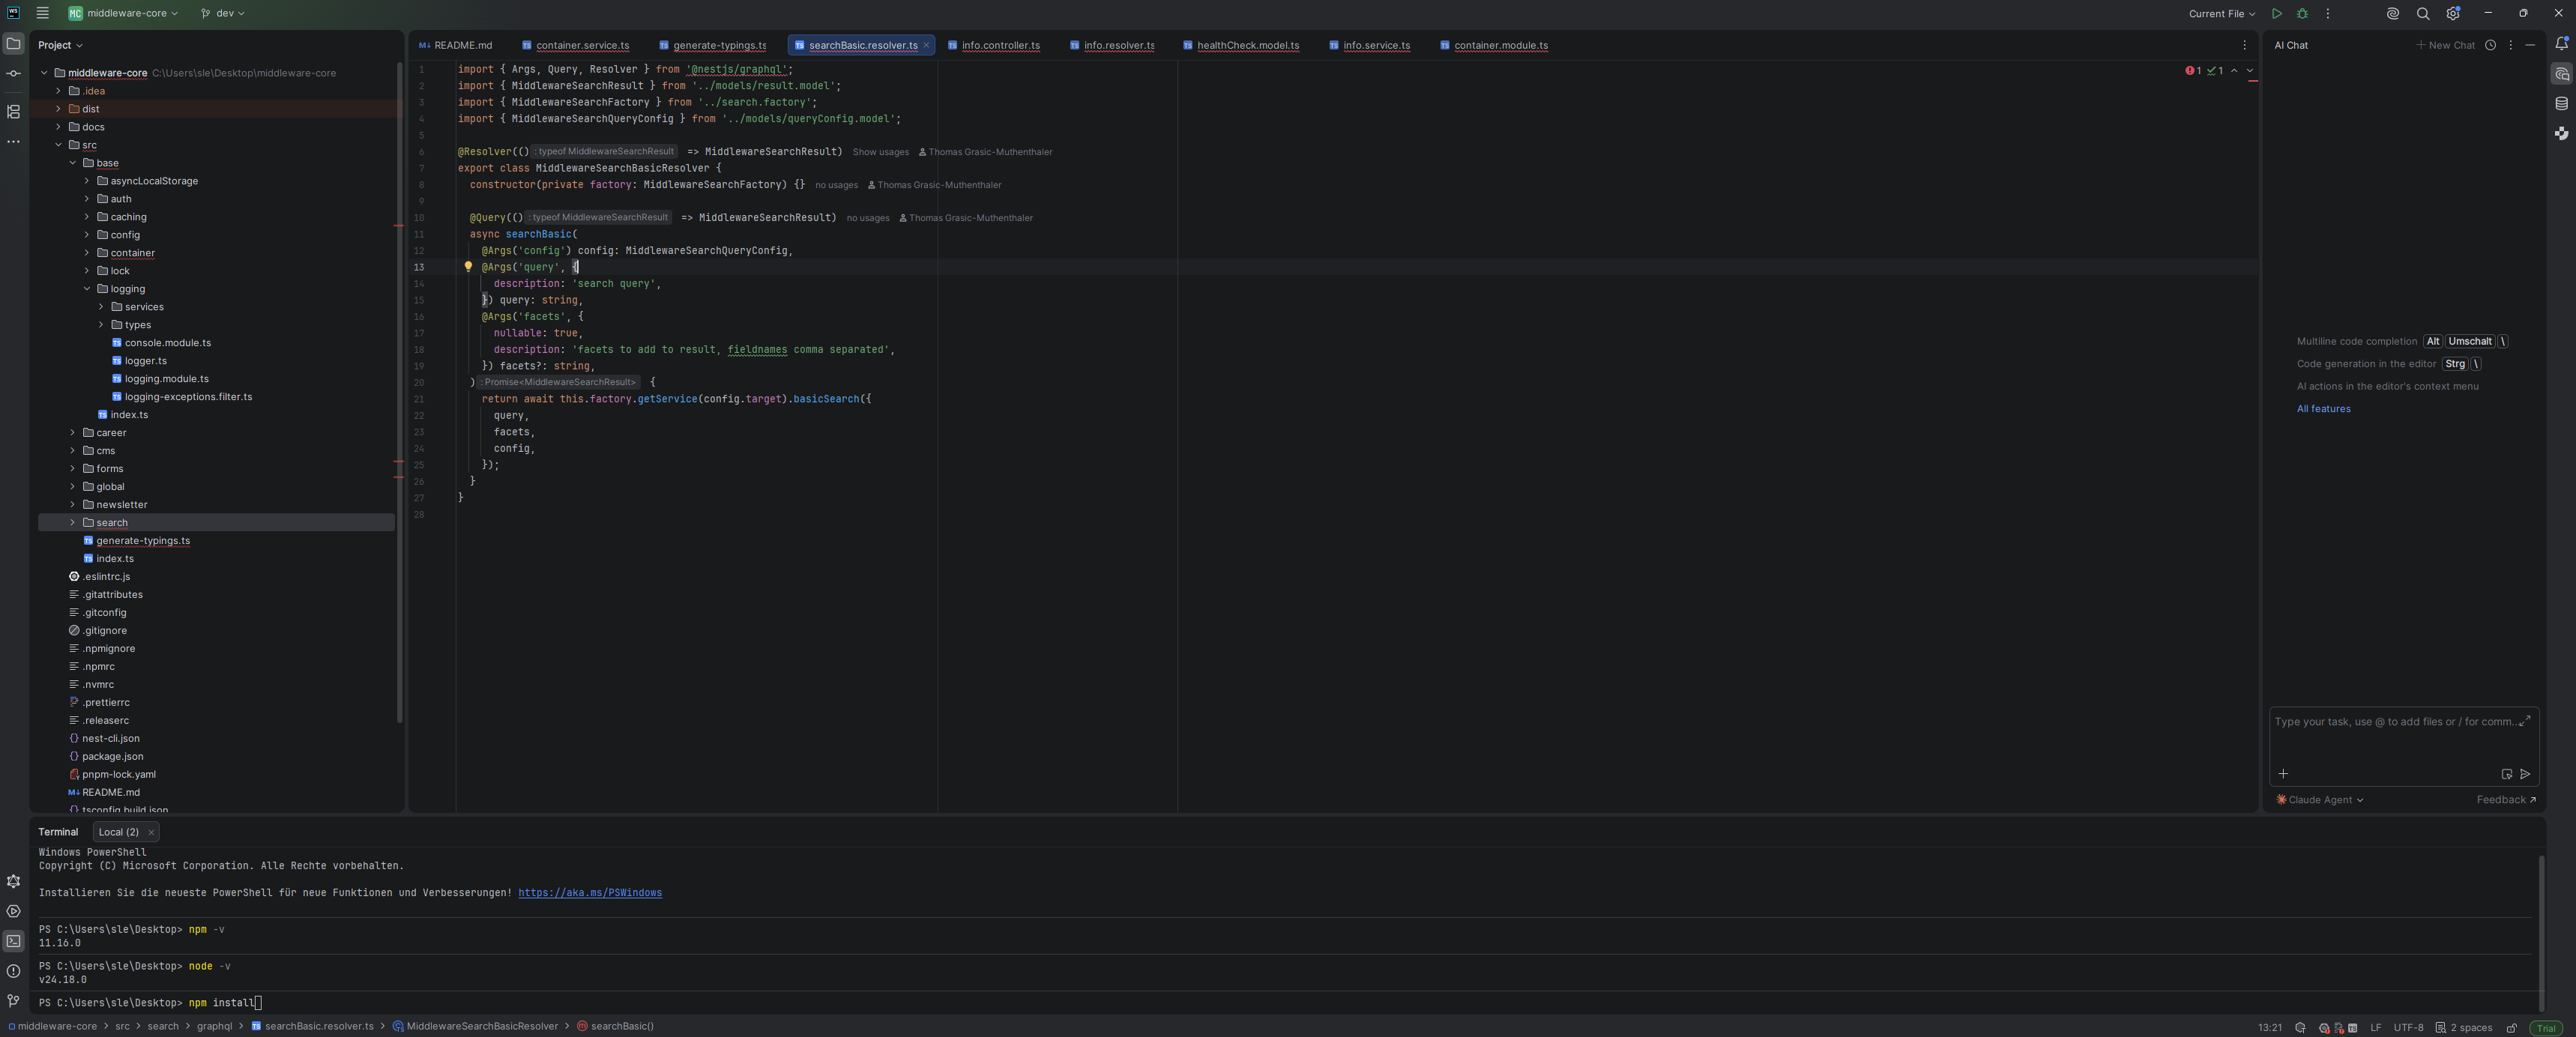
\includegraphics[width=0.9\textwidth, trim=0 0 975 0, clip]{webstorm-uebersicht.png}};
    \begin{scope}[x={(img.south east)}, y={(img.north west)}]
      % Namen in der Git-Blame-Anzeige abdecken
      \fill[black!70] (0.525,0.77) rectangle (0.66,0.865);
    \end{scope}
  \end{tikzpicture}
  \caption[Oberfläche von WebStorm]{WebStorm mit Projektbaum, Editor und Terminal, in dem mit \texttt{node -v} die Node-Version geprüft wird (eigener Screenshot, Namen unkenntlich gemacht)}
  \label{fig:webstorm}
\end{figure}

% ------------------------------------------------------------------
\section{Node.js und TypeScript}
\label{sec:node}
\label{sec:typescript}

\textbf{Node.js} ist eine Laufzeitumgebung, mit der JavaScript außerhalb des Browsers, etwa auf einem Server, ausgeführt werden kann~\cite{nodejs}. Node.js arbeitet \emph{nicht-blockierend}: Während ein Programm auf eine Antwort einer externen API wartet, bearbeitet es andere Anfragen weiter. Das passt gut zu einer Middleware, die hauptsächlich Anfragen an externe Dienste weiterleitet. Die LegoStack Middleware ist eine Node.js-Anwendung, und auch das Admin-Package läuft in ihrem Prozess.

\textbf{TypeScript} ist eine Erweiterung von JavaScript um \emph{statische Typen}~\cite{typescript}. Man legt fest, welchen Typ Variablen, Parameter und Rückgabewerte haben, und der Compiler prüft das vor dem Ausführen. Danach wird der Code in normales JavaScript übersetzt.

\begin{lstlisting}[language=TypeScript, caption={Typen in TypeScript}, label={lst:ts-typen}]
interface CacheInfo {
  type: string;
  size: number;
}
const info: CacheInfo = { type: 'memory', size: '12' };
// Fehler beim Kompilieren: '12' ist kein number
\end{lstlisting}

Für Kapitel~\ref{kap:architektur-iteration} ist wichtig: Typen und Interfaces gibt es \emph{nur beim Kompilieren}. Im fertigen JavaScript sind sie verschwunden. Ein Interface kann also beschreiben, welche Methoden eine Klasse hat, aber keine fehlende Methode hinzufügen.

% ------------------------------------------------------------------
\section{NestJS}
\label{sec:nestjs}

\textbf{NestJS} ist ein Framework für Serveranwendungen mit Node.js und TypeScript, auf dem die LegoStack Middleware aufbaut~\cite{nestjs}. Es arbeitet mit \emph{Decorators}, also Anmerkungen mit \texttt{@}, die Klassen und Methoden eine Rolle zuweisen~\cite{ts-decorators}. Die wichtigsten Bausteine sind:

\begin{description}
  \item[Module] fassen zusammengehörige Teile zusammen, z.\,B. alles zur Anmeldung~\cite{nestjs-modules}.
  \item[Services] enthalten die eigentliche Logik, etwa das Prüfen eines Passworts~\cite{nestjs-providers}.
  \item[Resolver / Controller] nehmen Anfragen entgegen, Resolver für GraphQL, Controller für REST.
  \item[Guards] entscheiden vor jeder Anfrage, ob sie bearbeitet werden darf~\cite{nestjs-guards}.
\end{description}

Ein zentrales Konzept ist \textbf{Dependency Injection}: Eine Klasse erzeugt die Objekte, die sie braucht, nicht selbst, sondern bekommt sie von NestJS über den Konstruktor übergeben (Codeausschnitt~\ref{lst:nest-di}). In Tests kann so statt des echten Services eine Attrappe (\emph{Mock}) übergeben werden.

\begin{lstlisting}[language=TypeScript, caption={Guard mit Dependency Injection (gekürzt aus \texttt{jwtUser.guard.ts})}, label={lst:nest-di}]
@Injectable()
export class JwtUserGuard implements CanActivate {
  // NestJS übergibt den Service automatisch
  constructor(private readonly adminAuthService: AdminAuthService) {}

  canActivate(context: ExecutionContext): boolean {
    // Token prüfen: true = weiter, sonst UnauthorizedException
  }
}
\end{lstlisting}

% ------------------------------------------------------------------
\section{pnpm}
\label{sec:pnpm}

Ein Paketmanager installiert die Bibliotheken, die in der \texttt{package.json} eines Projekts stehen, und hält die genauen Versionen in einer \emph{Lockfile} fest. \textbf{pnpm} speichert jede Paketversion nur einmal zentral auf dem Rechner und verlinkt sie in die Projekte, das spart Platz und Zeit~\cite{pnpm}. Verwendet wurden vor allem \texttt{pnpm install}, \texttt{pnpm build}, \texttt{pnpm start:dev}, \texttt{pnpm test} und \texttt{pnpm audit}. Pakete können auch direkt aus einem Git-Repository geladen werden, was im Projekt für die nicht öffentlichen LegoStack-Pakete genutzt wurde (Kapitel~\ref{kap:architektur-iteration}).

% ------------------------------------------------------------------
\section{Git, Bitbucket und SSH}
\label{sec:git}
\label{sec:ssh}

\textbf{Git} ist ein System zur Versionsverwaltung, das jeden Stand eines Projekts speichert~\cite{git}. Ein \emph{Repository} enthält das Projekt samt Versionsgeschichte, ein \emph{Commit} ist ein gespeicherter Stand, ein \emph{Branch} ein eigener Entwicklungszweig und ein \emph{Tag} ein fester Name für einen Commit, meist eine Versionsnummer wie \texttt{v0.1.1}. Abbildung~\ref{fig:git-areas} zeigt, wie eine Änderung vom Arbeitsverzeichnis über die Staging Area ins Repository gelangt.

\begin{figure}[htbp]
  \centering
  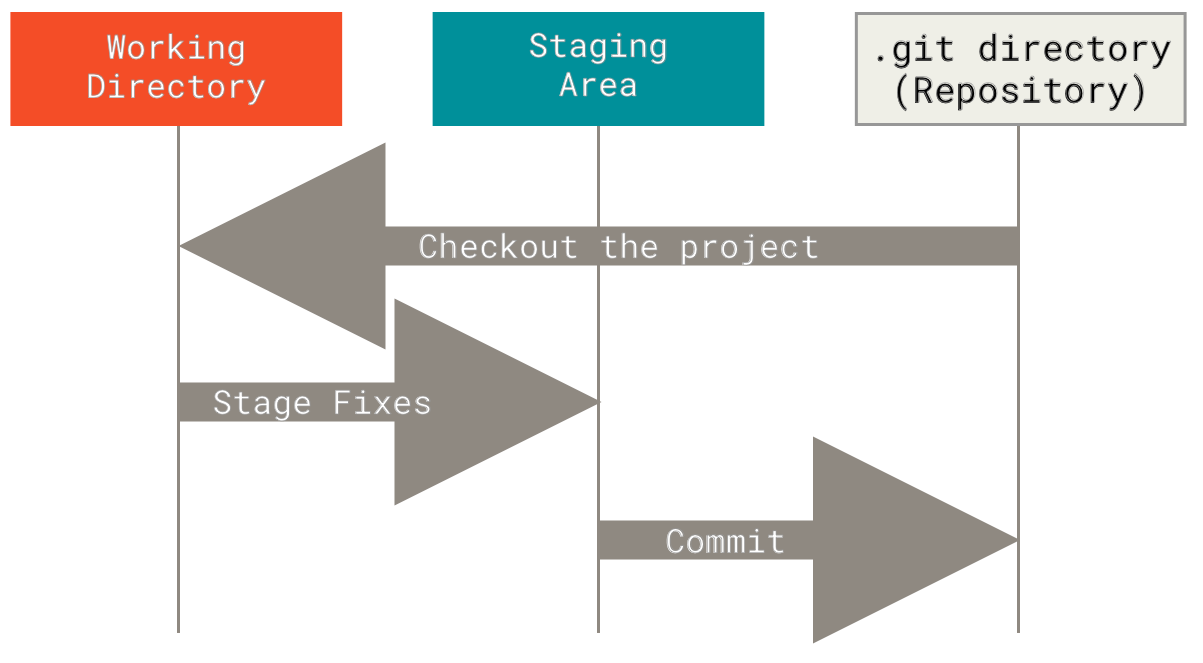
\includegraphics[width=0.6\textwidth]{git-areas.png}
  \caption[Die drei Bereiche von Git]{Die drei Bereiche von Git. Quelle: Chacon/Straub, \emph{Pro Git}~\cite{git}, Lizenz CC BY-NC-SA 3.0}
  \label{fig:git-areas}
\end{figure}

\textbf{Bitbucket} von Atlassian speichert Git-Repositorys zentral~\cite{bitbucket}. Änderungen werden dort über \emph{Pull Requests} eingereicht, die ein Kollege vor dem Übernehmen prüft (Code-Review). Alle Repositorys der LegoStack Middleware liegen auf Bitbucket, gearbeitet wurde auf dem Branch \texttt{dev}.

Für den Zugriff auf Bitbucket wird \textbf{SSH} (\emph{Secure Shell}) verwendet, ein Protokoll für verschlüsselte Verbindungen~\cite{ssh}. Statt eines Passworts nutzt man ein Schlüsselpaar: Der \emph{private Schlüssel} bleibt auf dem eigenen Rechner, der \emph{öffentliche Schlüssel} (\texttt{.pub}) wird bei Bitbucket hinterlegt. Bei der Anmeldung beweist der Rechner mit dem privaten Schlüssel seine Identität, ohne ihn zu übertragen (Abbildung~\ref{fig:ssh}). Umgekehrt prüft der Rechner anhand des \emph{Host Keys}, ob der Server echt ist, und merkt sich bekannte Server in der Datei \texttt{known\_hosts}~\cite{bitbucket-ssh}.

\begin{figure}[htbp]
  \centering
  \begin{tikzpicture}[
      box/.style={draw, rounded corners, fill=gray!10, minimum width=3.4cm, minimum height=1.1cm, align=center, font=\small},
      pfeil/.style={-{Stealth[length=2.5mm]}, thick}]
    \node[box] (pc) {Eigener Rechner\\ \footnotesize privater Schlüssel};
    \node[box, right=4cm of pc] (srv) {Bitbucket\\ \footnotesize öffentlicher Schlüssel};
    \draw[pfeil] ([yshift=3mm]pc.east) -- node[above, font=\footnotesize]{1. Verbindungswunsch} ([yshift=3mm]srv.west);
    \draw[pfeil] ([yshift=-1mm]srv.west) -- node[above, font=\footnotesize]{2. Aufgabe (Challenge)} ([yshift=-1mm]pc.east);
    \draw[pfeil] ([yshift=-5mm]pc.east) -- node[below, font=\footnotesize, align=center]{3. mit privatem Schlüssel\\ signierte Antwort} ([yshift=-5mm]srv.west);
  \end{tikzpicture}
  \caption[Anmeldung per SSH-Schlüssel]{Vereinfachter Ablauf der Anmeldung per SSH-Schlüssel (eigene Darstellung)}
  \label{fig:ssh}
\end{figure}

% ------------------------------------------------------------------
\section{REST und GraphQL}
\label{sec:rest}
\label{sec:graphql}

Programme kommunizieren im Web über \textbf{HTTP}: Ein Client schickt eine Anfrage, der Server antwortet mit Daten und einem Statuscode, z.\,B. \texttt{200} für Erfolg oder \texttt{401} für \enquote{nicht angemeldet}~\cite{mdn-http}. Bei \textbf{REST} hat jede Ressource eine eigene Adresse, und die HTTP-Methode (\texttt{GET}, \texttt{POST}, \texttt{PUT}, \texttt{DELETE}) gibt an, was passieren soll~\cite{rest-fielding}. Einige Wartungsfunktionen der Middleware, etwa das Auffrischen des Page-Caches, gab es bereits als REST-Endpunkte.

\textbf{GraphQL} hat dagegen nur \emph{einen} Endpunkt (\texttt{/graphql}). Was der Client möchte, steht in der Anfrage selbst, und er bekommt genau die angefragten Felder zurück~\cite{graphql}. Eine \textbf{Query} liest Daten, eine \textbf{Mutation} ändert etwas oder löst eine Aktion aus. Welche Operationen es gibt, legt das \textbf{Schema} fest. In NestJS werden Operationen in Resolvern mit Decorators wie \texttt{@Query()} geschrieben, und das Schema wird daraus automatisch erzeugt~\cite{nestjs-graphql}.

\begin{figure}[htbp]
  \centering
  \begin{tikzpicture}[
      scale=0.85, transform shape,
      box/.style={draw, rounded corners, fill=gray!10, minimum width=2.6cm, minimum height=0.8cm, align=center, font=\small},
      pfeil/.style={-{Stealth[length=2mm]}, thick}]
    \node[font=\small\bfseries] at (0,2.6) {REST};
    \node[box] (c1) at (0,1.5) {Client};
    \node[box, font=\footnotesize] (e1) at (4.2,2.4) {\texttt{GET /cache}};
    \node[box, font=\footnotesize] (e2) at (4.2,1.5) {\texttt{GET /health}};
    \node[box, font=\footnotesize] (e3) at (4.2,0.6) {\texttt{GET /logs}};
    \draw[pfeil] (c1.east) -- (e1.west);
    \draw[pfeil] (c1.east) -- (e2.west);
    \draw[pfeil] (c1.east) -- (e3.west);
    \node[font=\small\bfseries] at (8.2,2.6) {GraphQL};
    \node[box] (c2) at (8.2,1.5) {Client};
    \node[box, font=\footnotesize] (g) at (12,1.5) {\texttt{POST /graphql}\\ \scriptsize eine Anfrage};
    \draw[pfeil] (c2.east) -- (g.west);
  \end{tikzpicture}
  \caption[REST und GraphQL im Vergleich]{REST verteilt Daten auf viele Endpunkte, GraphQL bündelt alles über einen (eigene Darstellung)}
  \label{fig:rest-graphql}
\end{figure}

Zum Testen von GraphQL-Anfragen wurde die \textbf{Apollo Sandbox} verwendet~\cite{apollo-sandbox}. Sie liest das Schema der laufenden Anwendung ein, man kann darin Anfragen zusammenstellen, Header wie \texttt{Authorization} setzen und sieht sofort die Antwort (Abbildung~\ref{fig:apollo}). So wurde jede Operation geprüft, bevor das Frontend sie eingebunden hat.

\begin{figure}[htbp]
  \centering
  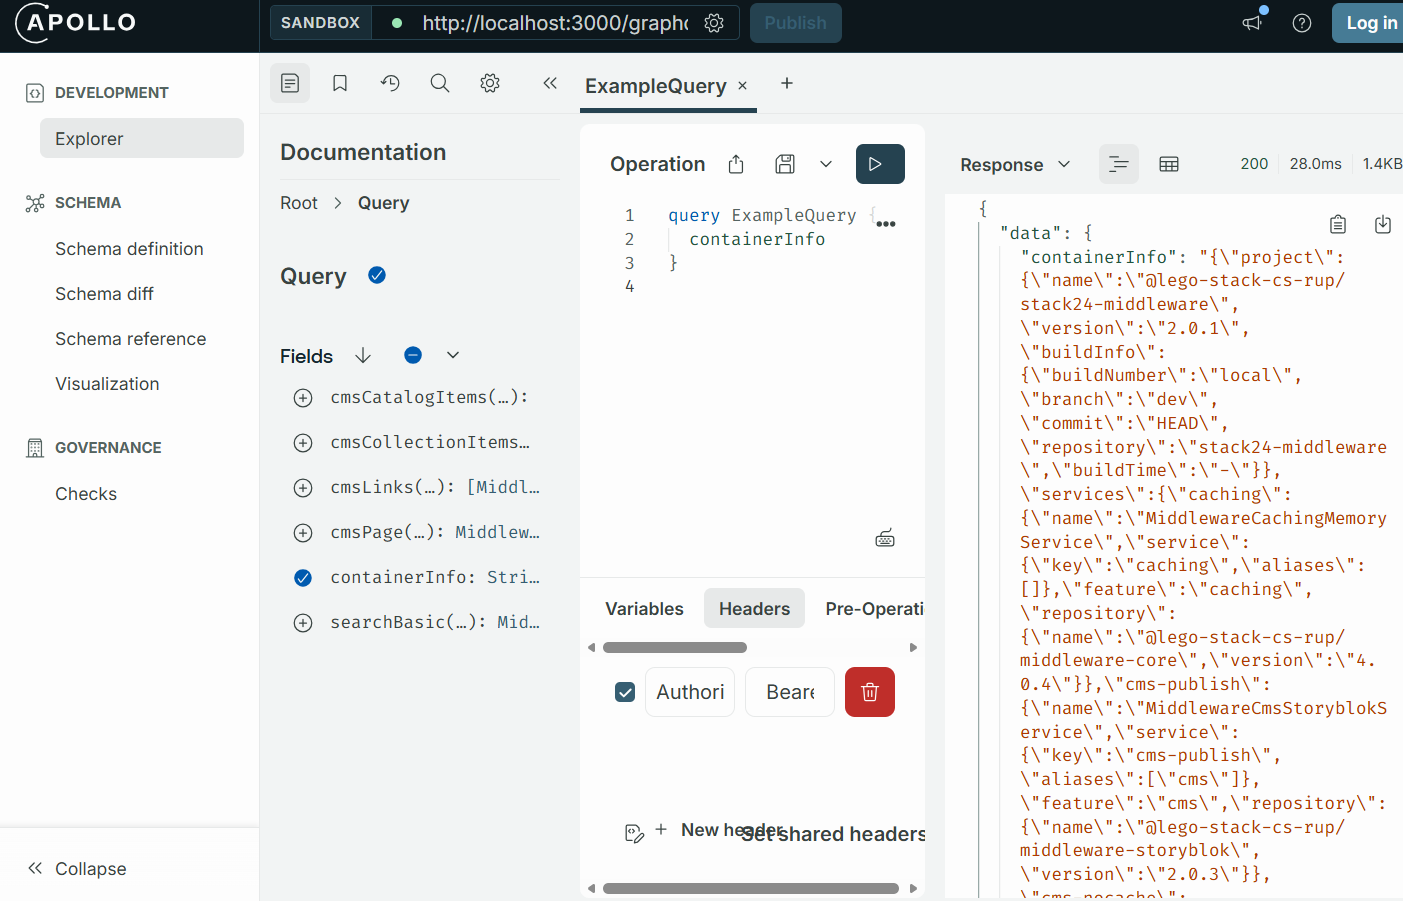
\includegraphics[width=0.75\textwidth]{apollo-sandbox-containerinfo.png}
  \caption[Apollo Sandbox]{Apollo Sandbox: links die Felder des Schemas, in der Mitte die Query \texttt{containerInfo} mit Header, rechts die Antwort (eigener Screenshot)}
  \label{fig:apollo}
\end{figure}

% ------------------------------------------------------------------
\section{Jira und Confluence}
\label{sec:jira}

\textbf{Jira} von Atlassian ist ein Werkzeug zur Aufgabenverwaltung~\cite{jira}. Jede Aufgabe ist ein \emph{Ticket} mit einem Status wie \enquote{To Do}, \enquote{In Arbeit} oder \enquote{Erledigt}. Im Projekt wurde zu jedem Ticket der aktuelle Stand mit einer kurzen Erklärung festgehalten, also was erledigt ist, was noch fehlt und woran es gerade hängt. Außerdem wurde die Arbeitszeit direkt auf die Tickets gebucht. So war für den Betreuer jederzeit sichtbar, wie weit eine Aufgabe ist.

\textbf{Confluence}, ebenfalls von Atlassian, ist ein Wiki für Dokumentation~\cite{confluence}. Dort wurden alle Liefergegenstände abgelegt, etwa die Stakeholder-Analyse, die Architecture Decision Records (Kapitel~\ref{kap:projektorganisation}) und die Übergabedokumentation. Da Confluence jede Änderung als Version speichert, ist nachvollziehbar, wie sich Entscheidungen im Lauf des Projekts verändert haben.

% ------------------------------------------------------------------
\section{Authentifizierung und Sicherheit}
\label{sec:sicherheit}

\subsection{JSON Web Tokens (JWT)}
\label{sec:jwt}

Ein \textbf{JSON Web Token} ist ein standardisiertes Format, mit dem ein Server bestätigt, wer ein Benutzer ist~\cite{rfc7519}. Nach dem Login stellt der Server ein Token aus, das der Client bei jeder Anfrage im Header \texttt{Authorization: Bearer <token>} mitschickt. Ein JWT besteht aus drei Teilen (Abbildung~\ref{fig:jwt})~\cite{jwt-io}. Header und Payload sind nur kodiert, nicht verschlüsselt, und dürfen daher keine Geheimnisse enthalten. Die Signatur stellt sicher, dass niemand den Inhalt unbemerkt verändern kann.

\begin{figure}[htbp]
  \centering
  \begin{tikzpicture}[
      teil/.style={draw, minimum height=1cm, align=center, font=\small},
      lbl/.style={font=\footnotesize, align=center}]
    \node[teil, fill=red!15, minimum width=3cm] (h) {Header};
    \node[right=0pt of h, font=\Large] (p1) {.};
    \node[teil, fill=violet!15, minimum width=4.5cm, right=0pt of p1] (p) {Payload};
    \node[right=0pt of p, font=\Large] (p2) {.};
    \node[teil, fill=cyan!15, minimum width=3cm, right=0pt of p2] (s) {Signatur};
    \node[lbl, below=2mm of h] {\texttt{\{"alg":"HS256"\}}};
    \node[lbl, below=2mm of p] {\texttt{\{"username":"admin",}\\ \texttt{"role":"admin","exp":...\}}};
    \node[lbl, below=2mm of s] {berechnet aus Header,\\ Payload und Secret};
  \end{tikzpicture}
  \caption[Aufbau eines JWT]{Aufbau eines JSON Web Tokens (eigene Darstellung nach~\cite{jwt-io})}
  \label{fig:jwt}
\end{figure}

Üblich ist die Kombination aus einem kurzlebigen \textbf{Access-Token} (z.\,B. 15 Minuten), der bei jeder Anfrage mitgeht, und einem langlebigen \textbf{Refresh-Token} (z.\,B. 7 Tage), mit dem nur neue Access-Tokens geholt werden. Ein gestohlener Access-Token ist so bald wertlos, ohne dass sich der Benutzer ständig neu anmelden muss.

\subsection{bcrypt und Rate Limiting}
\label{sec:bcrypt}
\label{sec:throttler}

Passwörter werden nie im Klartext gespeichert, sondern als \textbf{Hash}, aus dem sich das Passwort nicht zurückrechnen lässt. \textbf{bcrypt} ist ein Hash-Verfahren speziell für Passwörter~\cite{bcrypt-npm}: Es fügt einen zufälligen Wert (\emph{Salt}) hinzu und ist absichtlich langsam. Über den \emph{Cost-Faktor} lässt sich einstellen, wie aufwendig das Ausprobieren vieler Passwörter für einen Angreifer wird~\cite{owasp-password}.

\textbf{Rate Limiting} begrenzt, wie viele Anfragen ein Client pro Zeitspanne stellen darf, und schützt so den Login vor \emph{Brute-Force-Angriffen}. In NestJS übernimmt das das Paket \texttt{@nestjs/throttler} mit einem Guard, dem man Zeitspanne und Höchstzahl übergibt~\cite{nestjs-throttler}.

\subsection{CORS und Cookies}
\label{sec:cors-cookies}

Browser lassen eine Webseite nicht ohne Weiteres Anfragen an einen anderen \emph{Origin} (andere Domain oder anderer Port) schicken. Über \textbf{CORS} legt der Server fest, welche Origins zugreifen dürfen~\cite{mdn-cors}. \textbf{Cookies} speichert der Server im Browser, der sie bei jeder Anfrage automatisch mitschickt~\cite{mdn-cookies}. Für sensible Cookies gibt es drei wichtige Attribute:
\begin{itemize}
  \item \texttt{httpOnly}: JavaScript kann das Cookie nicht lesen, eingeschleuster Schadcode (XSS) kann es also nicht stehlen.
  \item \texttt{Secure}: Das Cookie wird nur über HTTPS übertragen.
  \item \texttt{SameSite}: Legt fest, ob das Cookie bei Anfragen von fremden Seiten mitgeschickt wird, und schützt so gegen CSRF. Für \texttt{SameSite=None} verlangen Browser zusätzlich \texttt{Secure}, was im Projekt beim Testen über zwei Rechner eine Rolle spielte (Kapitel~\ref{kap:architektur-iteration}).
\end{itemize}

% ------------------------------------------------------------------
\section{Weitere Bibliotheken und Werkzeuge}
\label{sec:weitere}
\label{sec:jest}
\label{sec:zod}
\label{sec:axios}
\label{sec:pm2}
\label{sec:figma}

Tabelle~\ref{tab:werkzeuge} fasst die übrigen verwendeten Werkzeuge zusammen. Wie sie eingesetzt wurden, beschreibt Kapitel~\ref{kap:implementierung}.

\begin{table}[htbp]
  \centering
  \small
  \begin{tabular}{p{2cm}p{10.4cm}}
    \hline
    \textbf{Werkzeug} & \textbf{Zweck im Projekt} \\
    \hline
    Jest & Test-Framework für Unit-Tests, bei NestJS standardmäßig dabei~\cite{jest,nestjs-testing}. Tests liegen als \texttt{.spec.ts} neben der getesteten Datei und werden mit \texttt{pnpm test} ausgeführt. \\
    Axios & Bibliothek für HTTP-Anfragen aus TypeScript~\cite{axios}. Damit ruft das Admin-Package vorhandene REST-Endpunkte der Middleware auf. \\
    Zod & Prüft Daten gegen ein Schema~\cite{zod}. Die Middleware prüft beim Start alle Umgebungsvariablen und startet bei fehlenden oder ungültigen Werten nicht. \\
    PM2 & Prozessmanager für Node.js im Produktivbetrieb~\cite{pm2}. Startet die Anwendung nach Abstürzen neu und liefert Uptime und Speicherverbrauch, die das Dashboard anzeigt. \\
    Figma & Browserbasiertes Design-Werkzeug~\cite{figma}. Damit wurden die Wireframes des Dashboards erstellt (Kapitel~\ref{kap:konzeption}). \\
    \hline
  \end{tabular}
  \caption{Weitere verwendete Bibliotheken und Werkzeuge}
  \label{tab:werkzeuge}
\end{table}
